% KHUNG ĐỊNH NGHĨA 2
\begin{tcolorbox}[
  enhanced,
  colback=white,
  colframe=stewartred,
  boxrule=0.8pt,
  arc=0mm,
  left=8pt,
  right=8pt,
  top=6pt,
  bottom=6pt
]
\noindent
\tikz[baseline=(n.base)]\node[draw=stewartred, line width=0.8pt, inner sep=2.5pt, font=\sffamily\bfseries\color{stewartred}] (n) {2};%
\hspace{6pt}{\sffamily\bfseries\color{stewartred} Định nghĩa}\quad
Một hàm số $f$ \textbf{liên tục bên phải tại một số $a$} nếu
\[
  \lim_{x \to a^+} f(x) = f(a)
\]
và $f$ \textbf{liên tục bên trái tại $a$} nếu
\[
  \lim_{x \to a^-} f(x) = f(a)
\]
\end{tcolorbox}

\vspace{6pt}

% VÍ DỤ 3
\noindent
{\bfseries\sffamily\color{stewartblue} VÍ DỤ 3}\quad Tại mỗi số nguyên $n$, hàm số $f(x) = \llbracket x \rrbracket$ [xem Hình 3(d)] liên tục bên phải nhưng gián đoạn bên trái vì
\[
  \lim_{x \to n^+} f(x) = \lim_{x \to n^+} \llbracket x \rrbracket = n = f(n)
\]
\noindent
nhưng
\begin{equation*}
  \lim_{x \to n^-} f(x) = \lim_{x \to n^-} \llbracket x \rrbracket = n - 1 \neq f(n)
  \tag*{\textcolor{stewartblue}{\rule{1.1ex}{1.1ex}}}
\end{equation*}

\vspace{6pt}

% KHUNG ĐỊNH NGHĨA 3
\begin{tcolorbox}[
  enhanced,
  colback=white,
  colframe=stewartred,
  boxrule=0.8pt,
  arc=0mm,
  left=8pt,
  right=8pt,
  top=6pt,
  bottom=6pt
]
\noindent
\tikz[baseline=(n.base)]\node[draw=stewartred, line width=0.8pt, inner sep=2.5pt, font=\sffamily\bfseries\color{stewartred}] (n) {3};%
\hspace{6pt}{\sffamily\bfseries\color{stewartred} Định nghĩa}\quad
Một hàm số $f$ \textbf{liên tục trên một khoảng} nếu nó liên tục tại mọi số thuộc khoảng đó. (Nếu $f$ chỉ được xác định về một phía tại một điểm mút của khoảng, ta hiểu \emph{liên tục tại điểm mút} có nghĩa là \emph{liên tục bên phải} hoặc \emph{liên tục bên trái}.)
\end{tcolorbox}

\vspace{6pt}

% VÍ DỤ 4
\noindent
{\bfseries\sffamily\color{stewartblue} VÍ DỤ 4}\quad Chứng minh rằng hàm số $f(x) = 1 - \sqrt{1 - x^2}$ liên tục trên đoạn $[-1, 1]$.

\vspace{2pt}
\noindent
{\bfseries\sffamily\color{stewartblue} LỜI GIẢI}\quad Nếu $-1 < a < 1$, khi đó sử dụng các Quy tắc Giới hạn từ Mục 2.3, ta có
\begin{align*}
  \lim_{x \to a} f(x) &= \lim_{x \to a} \left(1 - \sqrt{1 - x^2}\right) \\[4pt]
  &= 1 - \lim_{x \to a} \sqrt{1 - x^2} && \text{\color{annotblue}(theo các Quy tắc 2 và 8)} \\[4pt]
  &= 1 - \sqrt{\lim_{x \to a} (1 - x^2)} && \text{\color{annotblue}(theo 7)} \\[4pt]
  &= 1 - \sqrt{1 - a^2} && \text{\color{annotblue}(theo 2, 8 và 10)} \\[4pt]
  &= f(a)
\end{align*}

\noindent
Như vậy, theo Định nghĩa 1, $f$ liên tục tại $a$ nếu $-1 < a < 1$.% Khối hình ảnh lề trái
\marginpar{%
  \centering
  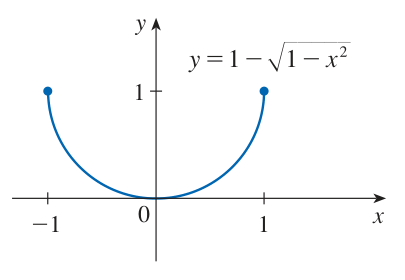
\includegraphics[width=\linewidth]{images/p0152_fig1.png}\par\vspace{3pt}
  {\footnotesize\sffamily\bfseries HÌNH 4}
}% Các phép tính tương tự cho thấy rằng
\[
  \lim_{x \to -1^+} f(x) = 1 = f(-1) \qquad \text{và} \qquad \lim_{x \to 1^-} f(x) = 1 = f(1)
\]
do đó $f$ liên tục bên phải tại $-1$ và liên tục bên trái tại $1$. Vì vậy, theo Định nghĩa 3, $f$ liên tục trên đoạn $[-1, 1]$.

Đồ thị của $f$ được phác họa trong Hình 4. Đó là nửa dưới của đường tròn
\begin{equation*}
  x^2 + (y - 1)^2 = 1
  \tag*{\textcolor{stewartblue}{\rule{1.1ex}{1.1ex}}}
\end{equation*}

\vspace{12pt}

% MỤC: TÍNH CHẤT CỦA CÁC HÀM SỐ LIÊN TỤC
\noindent
{\large\sffamily\bfseries\textcolor{stewartblue}{\rule{1.15ex}{1.15ex}}\hspace{0.5em}Tính chất của các hàm số liên tục}

\vspace{3pt}
\noindent
Thay vì luôn sử dụng các Định nghĩa 1, 2 và 3 để kiểm tra tính liên tục của một hàm số như chúng ta đã làm trong Ví dụ 4, việc sử dụng định lý tiếp theo thường thuận tiện hơn; định lý này chỉ ra cách xây dựng các hàm liên tục phức tạp từ những hàm đơn giản.
